\chapter{Introduction}
\section{The Problem}
One of the objectives of the SKA [Section \ref{ska}] is to create a comprehensive map of the sky as seen through radio wave signals. This can be achieved by taking long exposure images of the sky using its primary beam. However, these images are subject to errors. While a solution to correcting these issues has been found; it needs to be done in a way that is optimal to correct the errors in a reasonable amount of time.
%%%%%%%%%%%%%%%%%%%%%%%%%%%%%%%%%%%%%%%%%%%%%%%%%%%%%%%%%%%%%%%%%%%%%%%%%
%RESEARCH OBJCTIVES
%%%%%%%%%%%%%%%%%%%%%%%%%%%%%%%%%%%%%%%%%%%%%%%%%%%%%%%%%%%%%%%%%%%%%%%%%
\section{Research Objectives}
The main objective of this research paper is to create and implement a tessellation algorithm for determining the area over which the error needs to be corrected for each stellar element, given a sensitivity distribution, on the image and optimizing the algorithm to run as efficiently as possible.
%------------------------------------------------------------------------
\subsection{Basic Model}
A basic Voronoi Tessellation [Section \ref{tess}] algorithm will be created using the stellar elements as central points.
%------------------------------------------------------------------------
\subsection{First CPU Implementation}
The basic model will be written and implemented as sequential code to test it validity.
%------------------------------------------------------------------------
\subsection{Improved Model}
The tessellation algorithm will be improved to include the data given by the sensitivity distribution of the primary beam [Section \ref{tpb}].
%------------------------------------------------------------------------
\subsection{Second CPU Implementation}
The improved model will be rewritten implemented onto a CPU to test its validity.
%------------------------------------------------------------------------
\subsection{GPU Implementation}
The code will be ported to a GPU [Section \ref{gpu}] and rewritten for basic parallelism [Section \ref{parallel}]. The runtime of this will then be compared to that of the CPU code.
%------------------------------------------------------------------------
\subsection{Optimisation}
Both the code and the algorithm will be gradually improved for faster run times on a multiprocessor.
%%%%%%%%%%%%%%%%%%%%%%%%%%%%%%%%%%%%%%%%%%%%%%%%%%%%%%%%%%%%%%%%%%%%%%%%%
%Solution Methods
%%%%%%%%%%%%%%%%%%%%%%%%%%%%%%%%%%%%%%%%%%%%%%%%%%%%%%%%%%%%%%%%%%%%%%%%%
\newpage
\section{History and Background}
%------------------------------------------------------------------------
\subsection{The SKA}\label{ska}
The SKA project was started in order to create the world's largest array of radio telescopes. This will be achieved by having 197 radio telescopes situated in South Africa and Australia working together and covering an area close to one square kilometre. The array is set to have a resolution of over 50 times that of the Hubble Space Telescope while still covering massive areas of the sky \cite{SKAsite}.
%------------------------------------------------------------------------
\subsection{The Primary Beam}\label{tpb}
The primary beam is a mathematical function that describes the sensitivity pattern of an antenna. Naturally the beam is most sensitive in the centre of the direction in which it is facing, with fringes of sensitivity radiating out as can be seen in Figure \ref{beam}. The circular sensitivity present in Appendix \ref{beam} is also due to the fact that the telescope rotates in order to keep the centre of the beam focused on the same area of the sky. The errors produced by the lack of sensitivity in certain areas can be compensated for, but that lies outside the scope of this paper.
\begin{figure}[H]
	\centering
	\label{beam}
	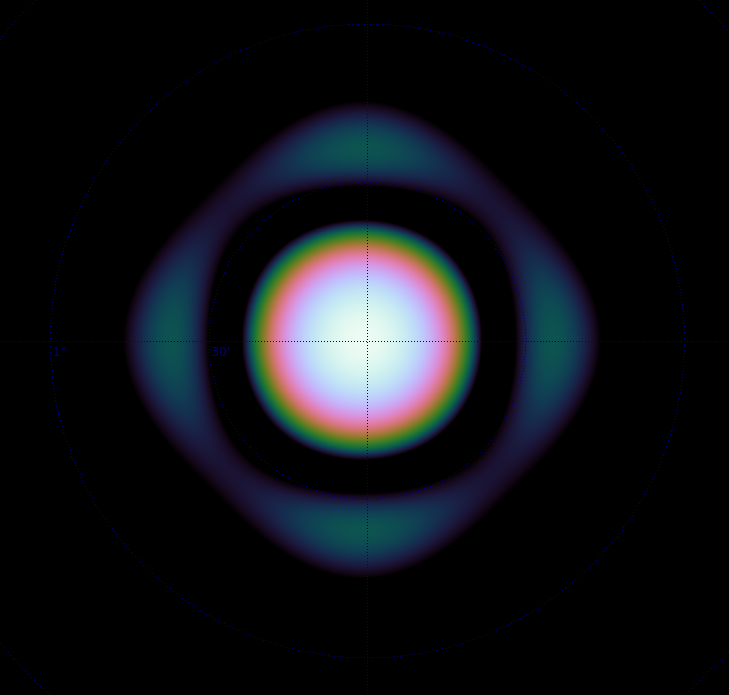
\includegraphics[scale=0.28]{Images/beam.png}
	\caption{Primary Beam Focus Pattern
\end{figure}
%------------------------------------------------------------------------
\subsection{Voronoi Diagrams}\label{tess}
A Voronoi Diagram is a partitioning of a space $S$ by a set of points. Given $n$ points the the space, $P = \{p_1,p_2,...,p_n\}, P \subset S$, is partitioned into $n$ regions, known as Voronoi Regions or Voronoi Cell, where every location, $s \in S_i,0 \leq i \leq n-1$ in a region, $S_i \subset S$, is closest to a single point, $p_i \in P$, in terms of the space's distance measurement operation, $d$ \cite{okabe2009spatial}. An example of a Voronoi Diagram can be seen in Appendix \ref{voronoipic}.
\begin{figure}[H]
	\centering
    \label{voronoipic}
    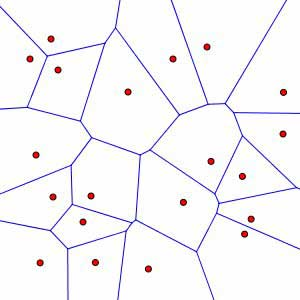
\includegraphics[scale=0.65]{Images/voronoi.jpg}
    \caption{Voronoi Diagram\cite{voronoipic}}
\end{figure}
%------------------------------------------------------------------------
\subsection{Parallelism}\label{parallel}
One of the main means of optimizing processing is through parallelism. The two main forms of parallelism are task and data parallelism. Task parallelism can be seen as running multiple processes concurrently where communication between the processes is explicitly defined to avoid race conditions. Data parallelism is the distribution of a data set over a number of identical processes each of which performs operations on a unique subset of the data. Race conditions occur when parallel processing streams access data or perform operations out of the intended order, leading to errors or incorrect output being produced. A combination of task and data parallelism can lead to an ideal speed-up, but both have their limits depending on the task and the data being operated on \cite{subhlok1993exploiting}.
\\
\\
The increased need for parallelism came in about 2005, when CPU frequency peaked at 4GHz due to heat dissipation issues. However, Moore's Law still holds, and is still expected to hold until 2025; that is, that the number of transistors for a computer will double every two years. This leads to a problem where the speed at which an operation is done cannot be increased (due to the frequency limit), but the number of concurrent operations can still increase. This means that the only way to speed up an operation is to change it from a sequential to a parallel process \cite{rajan2013informatics}.
%------------------------------------------------------------------------
\subsection{GPU Optimization}\label{gpu}
GPU's were originally designed for rendering pixels and vectors in games. They were especially designed for this since CPU's are optimized to run sequential instructions as fast as possible; whereas pixel and vector calculations are inherently parallel. With NVIDIA's release of CUDA in 2006, general purpose GPU (GPGPU) programming became common place as a way to accelerate data processing through data parallelism and task parallelism through the simultaneous execution of similar task \cite{nvidia_home}.
\\
\\
The power of GPU's come from its architecture which is optimized for a special case of SIMD (Single Instruction Multiple Data) processing known as SMIT (Single Instruction Multiple Threads). SIMD allows a central processor to distribute a set of instructions to multiple simple processors which then act on the data simultaneously. SIMT is more generalized as each thread of the GPU can perform different tasks given the same set of instructions. This is due to the way in which the GPU handles branching at the thread level. By exploiting these processes, and this instructional architecture, some instructions can be computed in faster time than that of a CPU \cite{vuduc2013brief}

%%%%%%%%%%%%%%%%%%%%%%%%%%%%%%%%%%%%%%%%%%%%%%%%%%%%%%%%%%%%%%%%%%%%%%%%%
%APPROACH
%%%%%%%%%%%%%%%%%%%%%%%%%%%%%%%%%%%%%%%%%%%%%%%%%%%%%%%%%%%%%%%%%%%%%%%%%
\section{Approach}
The research will be carried out by firstly determining a mathematical algorithm to obtain the Voronoi Tessellations [Section \ref{tess}] which best cover the image obtained given the primary beam's sensitivity distribution. Then the algorithm will be implemented into a sequential program which will be thoroughly tested to verify the tessellations process. The algorithm will then be implemented onto a multiprocessor, in this case a GPU [Section \ref{gpu}], to obtain a faster computation time through parallelism [Section \ref{parallel}].
%%%%%%%%%%%%%%%%%%%%%%%%%%%%%%%%%%%%%%%%%%%%%%%%%%%%%%%%%%%%%%%%%%%%%%%%%
%REQUIREMENTS AND RESOURCES
%%%%%%%%%%%%%%%%%%%%%%%%%%%%%%%%%%%%%%%%%%%%%%%%%%%%%%%%%%%%%%%%%%%%%%%%%
\section{Research Requirements}
The only necessary requirements for the project will be a modern computer with a GPU.
%%%%%%%%%%%%%%%%%%%%%%%%%%%%%%%%%%%%%%%%%%%%%%%%%%%%%%%%%%%%%%%%%%%%%%%%%
%TIMELINE
%%%%%%%%%%%%%%%%%%%%%%%%%%%%%%%%%%%%%%%%%%%%%%%%%%%%%%%%%%%%%%%%%%%%%%%%%
\section{Project Time-line}

\subsection{February - March 2016}
During this time research will be done into Voronoi Diagrams and the language to be used for the sequential implementation of the algorithm. The tessellation algorithm will begin to be formulated.

\subsection{April-May 2016}
The tessellation algorithm will be formulated to solve the problem. Research will be done on parallel processing and GPU processing. The literature review will be compiled and submitted by the end of May. Sequential implementation of the algorithm will begin.

\subsection{June - July 2016}
Time will be dedicated to the midyear exams and coursework projects. The tessellation algorithm will be tested as a sequential algorithm. More research will be done on GPU processing and parallel implementation will begin. The last 2 weeks of July will be dedicated mainly to coursework.

\subsection{August - September 2016}
The first 2 weeks of August will be dedicated mainly to coursework. The algorithm will be tested on a GPU for parallel processing. The algorithm will be iteratively optimised and retested both in the mathematical sense and in terms of the GPU. The final thesis write up will be compiled.

\subsection{October 2016}
The algorithm and its implementation will be continually optimised. The thesis will be completed and submitted by the end of October.
%%%%%%%%%%%%%%%%%%%%%%%%%%%%%%%%%%%%%%%%%%%%%%%%%%%%%%%%%%%%%%%%%%%%%%%%%